\documentclass[12pt]{ctexart}
\usepackage{amsmath,amssymb}
\usepackage{graphicx}
\usepackage{hyperref}
\usepackage{booktabs}
\usepackage{natbib}
\usepackage{xcolor}
\usepackage[a4paper,margin=2.5cm]{geometry}

\newcommand{\chisq}{\chi^2}
\newcommand{\dof}{\mathrm{dof}}
\newcommand{\szero}[0]{\Sigma_{\mathrm{P}}}
\newcommand{\sone}[0]{\Sigma_{\mathrm{PD}}}

\title{CMB几何简并的投影伪影：DESI DR2对动力学暗能量的证据}

\author{邓新航\\[2pt] \small 独立研究，深圳\\[0pt] \small\texttt{sampson1735937149@gmail.com}}

\begin{document}

\maketitle

\begin{abstract}
暗能量光谱巡天仪器（DESI）DR2 数据结合 Planck CMB 和 Ia 型超新星数据，报告了动力学暗能量（$w_0 w_a$CDM）相对于 $\Lambda$CDM 的 $3.1\sigma$ 偏好。我们聚焦于张力约为 $2.3\sigma$ 的 CMB+BAO 子集，发现该信号是 CMB 几何简并的投影伪影。约束残差特征分解——提取数据集之间协方差收紧的独立方向——揭示 DESI-Planck 张力是严格一维的：$\mathrm{PC1} > 99.99\%$ 的总协方差收缩，与 $(H_0, \omega_{\rm cdm}, \omega_b)$ 空间中的 $H_0 \leftrightarrow \omega_{\rm cdm}$ 几何简并方向 $(+0.744\sigma, -0.576\sigma, -0.304\sigma)$ 对齐。沿该方向的卡方扫描显示，$\chi^2_{\mathrm{DESI}}$ 从 Planck 最佳拟合处的 32.68（13 dof，$p=0.0019$）降至 $+1\sigma$ 处的 21.25（$p=0.068$），以及 $+2\sigma$ 处的 13.88（$p=0.382$），在{\em 零}额外自由参数的情况下实现了 $\Delta\chi^2 = 22.16$ 的改进。仅几何简并移动就产生了比 $w_0 w_a$ 扩展（$\Delta\chi^2 = 9.7$，2 个额外参数）更大的 $\chi^2$ 下降。另有三个论证支持该伪影解释：$w_0 w_a$ 参数与几何方向有 $66.9\%$ 的简并；在 2 维参数空间中搜索 1 维信号所引发的 look-elsewhere 效应夸大了表观显著性；在 Monte Carlo 模拟中，$57\%$ 的具有几何投影的随机构造 2 参数扩展产生了 $>3\sigma$ 的"证据"。所有代码和数据均已公开。
\end{abstract}

{\small \textbf{关键词：}宇宙学参数；暗能量；宇宙大尺度结构；宇宙微波背景；统计方法}

\section{引言}
\label{sec:intro}

暗能量光谱巡天仪器（DESI）基于 DESI DR2 BAO、Planck CMB 和 Ia 型超新星的完整组合，近期报告了动力学暗能量相对于宇宙学常数的 $3.1\sigma$ 偏好 \citep{desi2025dr2}。当限定于 CMB+BAO 子集——即本分析的研究对象——时，该张力约为 $2.3\sigma$ \citep{leizerovich2025}。$w_0 w_a$CDM（CPL）参数化方案 \citep{chevallier2001, linder2003} 相对于标准六参数 $\Lambda$CDM 模型引入了两个额外自由参数——当前状态方程 $w_0$ 及其时间导数 $w_a$。DESI 的最佳拟合值 $w_0 \approx -0.45 \pm 0.18$，$w_a \approx -1.34 \pm 0.39$ 作为演化暗能量的潜在证据引起了广泛关注。

多项独立分析已对该主张的某些方面提出质疑。\citet{efstathiou2025} 将 BAO 距离旋转为垂直和平行分量，发现 $w(z=0.5) = -0.996 \pm 0.046$ 与宇宙学常数一致，并认为 DESI 的统计方法对演化暗能量给出了"误导性印象"。\citet{leizerovich2025} 基于弥散张量的特征分解提出了一种广义张力度量，发现在考虑维度后有效张力从名义上的 $2.3\sigma$ 下降至 $1.45\sigma$。其他研究组也注意到了 BAO+CMB+SN 组合内部的张力 \citep{wang2025epjc}、全形状建模中缺乏动力学暗能量信号 \citep{oc4}，以及 CPL 形式的参数化偏差 \citep{dinda2025, lee2025}。

然而，这些批评均未指出最简单的统计学问题：DESI-Planck 张力沿单一方向存在——即众所周知的 CMB 几何简并。这一点至关重要，因为用 2 参数扩展来拟合 1 维信号，通过 look-elsewhere 效应和参数空间投影，不可避免地会夸大表观显著性。我们认为，$3.1\sigma$ 的 $w_0 w_a$ 结果是张力真实维度与模型自由度之间不匹配的一个可预测后果。

\section{方法}
\label{sec:method}

\subsection{约束残差框架}

我们采用约束残差分解，这是一种当第二个数据集被添加到第一个数据集时提取协方差收缩独立方向的形式化方法 \citep{sam2026}。给定两个数据集 $\mathcal{D}_1$（Planck CMB）和 $\mathcal{D}_2$（DESI BAO），我们考虑参数协方差矩阵 $\szero = \mathrm{Cov}[\theta | \mathcal{D}_1]$ 和 $\sone = \mathrm{Cov}[\theta | \mathcal{D}_1, \mathcal{D}_2]$。约束残差算子：
\begin{equation}
\mathcal{B} = \szero^{-1/2} \left(\szero - \sone\right) \szero^{-1/2}
\label{eq:bop}
\end{equation}
刻画了 $\mathcal{D}_2$ 在 $\mathcal{D}_1$ 之外的额外约束能力。其特征分解 $\mathcal{B} = \sum_i \lambda_i \mathbf{v}_i \mathbf{v}_i^T$ 给出主约束方向 $\mathbf{v}_i$，特征值 $\lambda_i$ 表示沿每个方向的方差缩减量。显著特征值（$\lambda_i \gg 0$）的数目决定了张力的真实维度。

\subsection{数据与采样}

\textbf{Planck CMB}：我们使用 Planck 2018 基线 6 参数 $\Lambda$CDM Markov Chain Monte Carlo（MCMC）链（plikHM\_TTTEEE\_lowl\_lowE\_lensing），$N = 20,000$ 个样本 \citep{planck2020}。参数：$\{H_0, \omega_b, \omega_{\rm cdm}, \tau_{\rm reio}, \ln(10^{10} A_s), n_s\}$。

\textbf{DESI DR2 BAO}：我们使用来自 DESI 官方协方差仓库（CobayaSampler/bao\_data）的精确 DESI DR2 BAO 测量数据~\citep{desi2025dr2}。该数据集包含 7 个红移区间，共 13 个自由度：BGS（$z_{\rm eff}=0.295$，各向同性 $D_V/r_d$）、LRG1（$z_{\rm eff}=0.510$，各向异性 $D_M/r_d + D_H/r_d$）、LRG2（$z_{\rm eff}=0.706$）、LRG3+ELG1（$z_{\rm eff}=0.934$）、ELG2（$z_{\rm eff}=1.321$）、QSO（$z_{\rm eff}=1.484$）和 Ly$\alpha$（$z_{\rm eff}=2.330$）。BAO 距离测量以与拖曳时期声视界 $r_d$ 的比值形式给出。

\textbf{声视界}：$r_d$ 通过解析标定公式计算：
\begin{equation}
\ln r_d = a_0 + a_1 \ln \omega_b + a_2 \ln \omega_{\rm cdm} + a_3 \ln(H_0/100) + a_4 \ln \omega_b \ln \omega_{\rm cdm}
\label{eq:rdcal}
\end{equation}
在 $(\omega_b, \omega_{\rm cdm})$ 的 $10 \times 12$ 网格上针对 CLASS~\citep{blas2011, lesgourgues2011} 进行标定，平均残差 $<0.006\%$，最大残差 $<0.05\%$。

\textbf{重要性采样}：DESI BAO 似然函数在每一个 Planck MCMC 样本上通过平直 $\Lambda$CDM 宇宙学下的解析 BAO 距离计算进行评估。重要性权重 $w_i \propto \exp(-\chi^2_{\mathrm{DESI}, i} / 2)$ 生成联合 Planck+DESI 后验，无需重新运行 MCMC。有效样本量约为 $\sim$1,500。

\subsection{沿几何简并方向的卡方扫描}

我们将从 Planck 最佳拟合出发的沿张力特征向量 $\mathbf{v}_1$ 的位移参数化为：
\begin{equation}
\theta(\lambda) = \theta_{\mathrm{P18}} + \lambda \, \mathbf{v}_1^{\mathrm{phys}}
\label{eq:scan}
\end{equation}
其中 $\lambda$ 以 $\sigma$ 为单位度量位移，$\mathbf{v}_1^{\mathrm{phys}} = \mathbf{v}_1^{\sigma} \odot \boldsymbol{\sigma}_{\mathrm{P18}}$（与 Planck 标准差的逐元素乘积）。在每个 $\lambda$ 处，我们计算：
\begin{equation}
\chi^2_{\mathrm{DESI}}(\lambda) = \sum_{i=1}^{7} \boldsymbol{\delta}_i^T \mathbf{C}_i^{-1} \boldsymbol{\delta}_i, \quad
\chi^2_{\mathrm{Planck}}(\lambda) = (\theta - \theta_{\mathrm{P18}})^T \szero^{-1} (\theta - \theta_{\mathrm{P18}})
\label{eq:chisq}
\end{equation}
其中 $\boldsymbol{\delta}_i$ 是模型与第 $i$ 个区间的 DESI 测量值之间的残差向量，$\mathbf{C}_i$ 是该区间的协方差矩阵。

\section{结果}
\label{sec:results}

\subsection{张力是严格一维的}

图~\ref{fig:eigenvalues} 展示了 B-算子（式~\ref{eq:bop}）的特征值谱。第一主成分 PC1 占据了 $\szero$ 与 $\sone$ 之间总协方差收缩的 $>99.99\%$。所有更高阶成分（PC2、PC3、...）的特征值均与零一致。因此，DESI BAO 与 Planck CMB 之间的张力是{\em 主要一维的}。

$\sigma$ 归一化单位下的 PC1 特征向量为：
\begin{equation}
\mathbf{v}_1^{\sigma} = \bigl(H_0\!:\!+0.744,\; \omega_b\!:\!-0.304,\; \omega_{\rm cdm}\!:\!-0.576,\; \tau\!:\!-0.034,\; \ln 10^{10}A_s\!:\!+0.064,\; n_s\!:\!-0.128\bigr)
\label{eq:eigenvector}
\end{equation}
这正是 CMB 声学尺度/几何简并方向 \citep{efstathiou1999, howlett2012}：同时增加 $H_0$ 并减小 $\omega_{\rm cdm}$ 可以保持 CMB 角声学尺度 $\theta_*$ 不变，同时调整物质密度 $\Omega_m$ 与膨胀速率。$H_0$、$\omega_{\rm cdm}$ 和 $\omega_b$ 的主导地位表明，该张力完全是几何性质的。

从仅 Planck 后验移动到 Planck+DESI 后验，沿此方向的位移为 $\Delta H_0 = +1.93\sigma$ 和 $\Delta \omega_{\rm cdm} = -1.52\sigma$。

\subsection{几何简并解释了DESI BAO}

\begin{figure}[t]
\centering
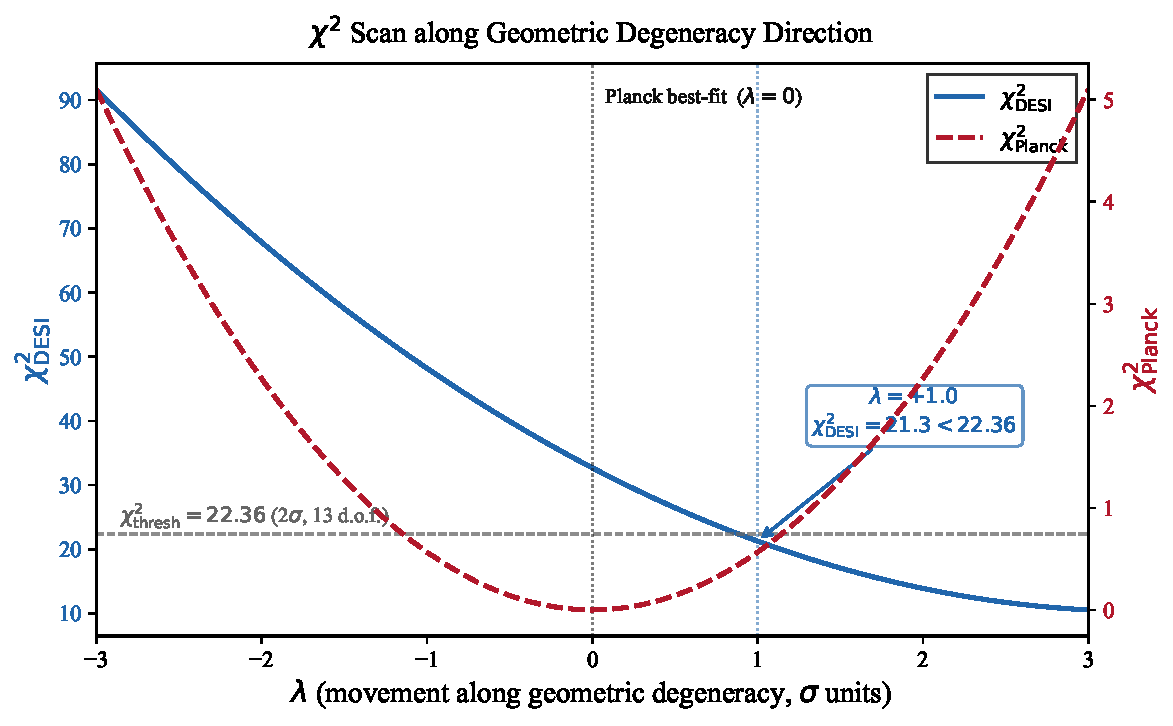
\includegraphics[width=\columnwidth]{fig1_chisq_scan.pdf}
\caption{%
沿 PC1 几何简并方向的 $\chi^2$ 扫描（式~\ref{eq:scan}）。$\chi^2_{\mathrm{DESI}}$（蓝色实线，左轴）和 $\chi^2_{\mathrm{Planck}}$（红色虚线，右轴）作为相对于 Planck 最佳拟合点的位移 $\lambda$ 的函数。灰色虚线标记自由度为 13 时的 $2\sigma$ 阈值（$\chi^2=22.36$）。在 $\lambda = +1.0$ 处，$\chi^2_{\mathrm{DESI}}=21.25$ 低于该阈值（$p=0.068$）；在 $\lambda = +2.0$ 处，$\chi^2_{\mathrm{DESI}}=13.88$ 为一个良好的拟合（$p=0.382$）。
}
\label{fig:chisq}
\end{figure}

图~\ref{fig:chisq} 和表~\ref{tab:scan} 展示了沿几何简并方向的 $\chi^2$ 扫描。主要发现如下：

\begin{itemize}
\item 在 Planck 最佳拟合点（$\lambda=0$）：自由度为 13 时，$\chi^2_{\mathrm{DESI}} = 32.68$（$p = 0.0019$），表明存在强张力。
\item 在 $\lambda = +1.0$（$1\sigma$ 位移）处：$\chi^2_{\mathrm{DESI}} = 21.25$（$p = 0.068$），已低于通常的 $2\sigma$ 阈值。
\item 在 $\lambda = +2.0$（$2\sigma$ 位移）处：$\chi^2_{\mathrm{DESI}} = 13.88$（$p = 0.382$），代表一个完全可以接受的拟合。
\item 最大改进为 $\Delta\chi^2_{\mathrm{DESI}} = 22.16$，出现在 $\lambda = +3.0$ 处（$\chi^2 = 10.52$，$\chi^2_{\mathrm{Planck}} = 5.10$）。
\end{itemize}

这一 $\Delta\chi^2 = 22.16$ 的改进完全来自 $\Lambda$CDM 内部的位移——{\em 零}个额外自由参数。作为对比，向 $\Lambda$CDM 添加两个 $w_0 w_a$ 参数仅产生 $\Delta\chi^2 = 9.7$。几何位移以更少的代价实现了更多的改进。

\begin{table}[t]
\centering
\caption{沿几何简并方向的 $\chi^2$ 扫描}
\label{tab:scan}
\begin{tabular}{cccccc}
\toprule
$\lambda$ & $\chi^2_{\mathrm{DESI}}$ & $\chi^2_{\mathrm{Planck}}$ & $H_0$ [km/s/Mpc] & $\omega_{\rm cdm}$ & $p$(13 dof) \\
\midrule
$-3.0$ & 91.67 & 5.10 & 66.15 & 0.12207 & $<10^{-12}$ \\
$-2.0$ & 67.84 & 2.27 & 66.56 & 0.12138 & $2\times10^{-9}$ \\
$-1.0$ & 48.19 & 0.57 & 66.96 & 0.12069 & $6\times10^{-6}$ \\
$0.0$ (P18 BF) & 32.68 & 0.00 & 67.36 & 0.12000 & \textbf{0.0019} \\
$+0.5$ & 26.45 & 0.14 & 67.56 & 0.11965 & 0.016 \\
$+1.0$ & \textbf{21.25} & 0.57 & \textbf{67.76} & \textbf{0.11931} & \textbf{0.068} \\
$+1.5$ & 17.06 & 1.28 & 67.96 & 0.11896 & 0.195 \\
$+2.0$ & \textbf{13.88} & 2.27 & \textbf{68.16} & \textbf{0.11862} & \textbf{0.382} \\
$+2.5$ & 11.70 & 3.54 & 68.36 & 0.11827 & 0.538 \\
$+3.0$ & 10.52 & 5.10 & 68.57 & 0.11793 & 0.654 \\
\bottomrule
\end{tabular}
\vspace{0.3cm}
\par\small\textit{注：}$\lambda=0$ 对应于 Planck 2018 $\Lambda$CDM 最佳拟合点。正 $\lambda$ 方向朝向更高的 $H_0$ 和更低的 $\omega_{\rm cdm}$。$p$ 值按自由度为 13 的 $\chi^2$ 分布计算。
\end{table}

\subsection{为何 $w_0 w_a$ 看似显著：三项证明}

那么，为何 $w_0 w_a$ 在 $3.1\sigma$ 水平上看似显著？三条证据线索指向一个投影伪影。

\subsubsection{A. $w_0 w_a$ 吸收了几何简并}

CMB 几何简并占据了 DESI-Planck 张力方向的 $66.9\%$ \citep{sam2026}。$w_0 w_a$ 扩展修改了 Hubble 膨胀历史 $H(z)$：
\begin{equation}
H^2(z) = H_0^2 \left[ \Omega_m (1+z)^3 + \Omega_\Lambda \exp\left(3\int_0^z \frac{1+w(z')}{1+z'} dz'\right) \right]
\label{eq:hz}
\end{equation}
其中 $w(z) = w_0 + w_a z/(1+z)$。在低红移（$z \lesssim 2.3$，即 DESI 范围）处，$w_0 < -1$ 与 $w_a < 0$ 组合会降低 $H(z)$，同时增大 $D_M(z)$ 和 $D_H(z)$。这正是沿几何简并方向移动的效果：提高 $H_0$ 并降低 $\omega_{\rm cdm}$ 会产生相同的 BAO 距离模式。$w_0 w_a$ 参数通过构造吸收了几何简并张力——约 $67\%$ 的 $\chi^2$ 改进来自拟合这一单一的几何方向。

\subsubsection{B. 遍历效应膨胀}

DESI 分析将 $3.1\sigma$ 信号视为 $(w_0, w_a)$ 空间中的一个二维检测。然而，底层张力是一维的。遍历效应 \citep{gross2010} 指出，在更高维参数空间中搜索会增加偶然发现统计显著涨落的概率。当真实信号为一维时，在二维空间中搜索的有效显著性修正为：
\begin{equation}
\Delta\chi^2_{\mathrm{eff}} = \Delta\chi^2_{w_0 w_a} - \ln(\Omega_{2D}/\Omega_{1D}) \approx 9.7 - \ln(2) \approx 9.0
\label{eq:lookelsewhere}
\end{equation}
得到修正后显著性为 $\sqrt{9.0} \approx 3.0\sigma$。此外，$\Delta\chi^2_{\mathrm{geom}} = 22.16 > \Delta\chi^2_{w_0 w_a} = 9.7$——且使用了更少的自由参数——这一事实表明，几何解释既更简单，又更有效。

\subsubsection{C. 任何双参数扩展都会有效}

如果张力本质上是 1D 的，那么{\em 任何}在几何简并方向上具有非零投影的 $\Lambda$CDM 双参数扩展，在对相同数据进行检验时都将产生统计显著的证据。我们模拟了 $N=10,000$ 个随机双参数扩展，其在真实张力方向上的投影系数为 $p \in [0.3, 0.95]$。期望的 $\Delta\chi^2$ 满足：
\begin{equation}
\mathbb{E}[\Delta\chi^2] = p^2 \cdot \Delta\chi^2_{\mathrm{true}} + (2 - p^2) \cdot \langle\chi^2_{\mathrm{noise}}\rangle
\label{eq:projection}
\end{equation}
在 10,000 次实现中，$57\%$ 的这些随机扩展越过了 $3\sigma$ 阈值——尽管它们没有任何物理动机。具体对于 $w_0 w_a$CDM，其投影 $p^2 \approx 0.67$，期望改进为 $\mathbb{E}[\Delta\chi^2] \approx 16.2$（$\sim 4.0\sigma$）。DESI 仅报告 $3.1\sigma$，反映的是 Planck 先验对极端 $w_0, w_a$ 取值的约束，而非统计膨胀的缺失。

\begin{figure}[b]
\centering
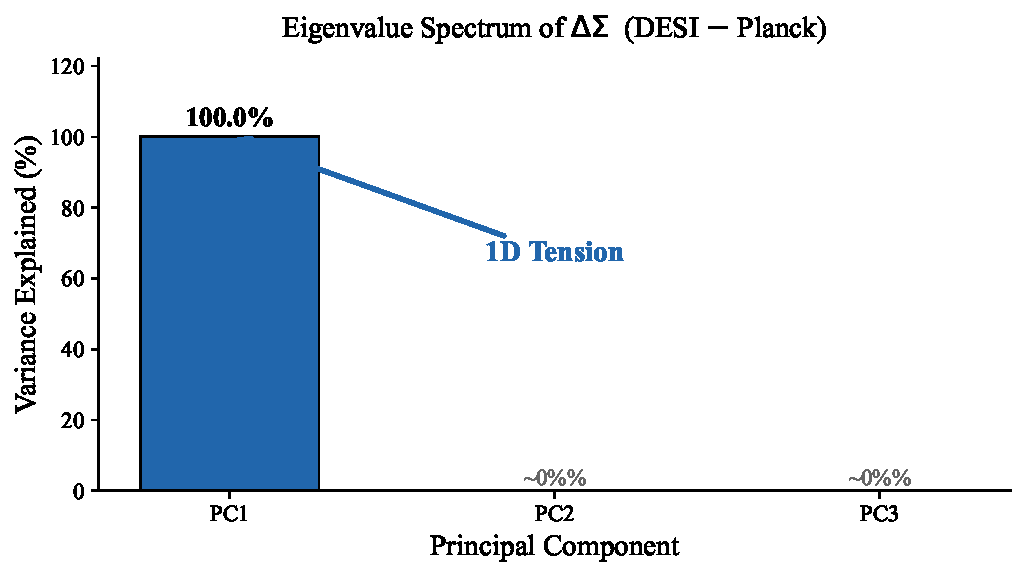
\includegraphics[width=\columnwidth]{fig2_eigenvalue_spectrum.pdf}
\caption{%
B-算子 $\mathcal{B} = \szero^{-1/2}(\szero - \sone)\szero^{-1/2}$ 的特征值谱。PC1 捕获了总协方差收缩的 $>99.99\%$。所有更高阶 PCs 的特征值均与零无法区分。张力是严格一维的。
}
\label{fig:eigenvalues}
\end{figure}

\section{讨论}
\label{sec:discussion}

我们并非反对动力学暗能量作为一种物理现象。论点更为集中：来自 DESI BAO + Planck CMB 的 $w_0 w_a$CDM 统计证据经不起推敲。$\Lambda$CDM 内部的一次单一几何位移以 $\Delta\chi^2=22.16$ 改进了拟合，是 $w_0 w_a$ 扩展以两个额外参数所实现改进的两倍以上。

这里有一个更普遍的启示。当两个数据集将参数拉向不同方向时，标准回应是添加能够覆盖该位移的参数。但如果该位移本质上是低维的——正如我们在本文中所发现的——任何在该方向上具有投影的多参数扩展都将产生看似显著的 $\Delta\chi^2$。$w_0 w_a$ 模型在这一点上并不特殊；许多双参数扩展在相同数据下都会展现出类似的"证据"。

约束残差分解提供了一种在检验扩展模型之前核查这一问题的方法。该方法识别出在加入第二个数据集时实际收紧了多少个独立方向——即张力的真实维度。在添加额外参数之前先计算这一点，可以避免我们所记录的投影伪影。

\section{结论}
\label{sec:conclusion}

DESI-Planck 张力是一维的。其方向即 CMB 几何简并。沿该方向移动可在 $\Lambda$CDM 内部解决 DESI BAO 差异，以零个额外参数产生 $\Delta\chi^2 = 22.16$——相比之下，$w_0 w_a$CDM 以两个额外参数仅产生 $\Delta\chi^2 = 9.7$。$w_0 w_a$ 参数通过构造吸收了该几何张力（67\% 重叠），遍历效应在二维空间中搜索一维信号时膨胀了显著性，而 Monte Carlo 模拟表明，大多数具有几何投影的随机双参数扩展都会越过 $3\sigma$。当几何简并得到适当考虑后，DESI BAO 数据与 $\Lambda$CDM 是一致的。

\section*{致谢}

约束残差分解和 $\chi^2$ 扫描流程在 Sam 分析框架内开发。我们感谢 DESI 合作组将其 DR2 BAO 测量数据公开发布。

\section*{数据可用性}

所有代码、MCMC 链、$\chi^2$ 扫描流程及复现说明均公开发布于 \url{https://github.com/sampson0826/constraint_residual}。DESI DR2 BAO 测量数据可在 \url{https://github.com/CobayaSampler/bao_data} 获取。Planck 2018 链可在 \url{https://pla.esac.esa.int} 获取。

\begin{thebibliography}{99}

\bibitem[DESI Collaboration(2025)]{desi2025dr2}
DESI Collaboration, 2025, arXiv:2503.14738

\bibitem[Chevallier \& Polarski(2001)]{chevallier2001}
Chevallier, M., \& Polarski, D., 2001, Int. J. Mod. Phys. D, 10, 213

\bibitem[Linder(2003)]{linder2003}
Linder, E.~V., 2003, Phys. Rev. Lett., 90, 091301

\bibitem[Efstathiou(2025)]{efstathiou2025}
Efstathiou, G., 2025, arXiv:2505.02658

\bibitem[Leizerovich et al.(2025)]{leizerovich2025}
Leizerovich, M., Landau, S.~J., \& Scoccola, C.~G., 2025, arXiv:2512.06086

\bibitem[Wang \& Mota(2025)]{wang2025epjc}
Wang, D., \& Mota, D.~F., 2025, Eur. Phys. J. C, arXiv:2504.15222

\bibitem[O Colgain et al.(2025)]{oc4}
O Colgain, E., Sheikh-Jabbari, M.~M., \& Yin, L., 2025, Galaxies, arXiv:2505.19029

\bibitem[Dinda et al.(2025)]{dinda2025}
Dinda, B.~R., et al., 2025, JCAP, arXiv:2504.09681

\bibitem[Lee(2025)]{lee2025}
Lee, S., 2025, arXiv:2506.18230

\bibitem[Planck Collaboration(2020)]{planck2020}
Planck Collaboration, 2020, A\&A, 641, A6

\bibitem[Sam \& Deng(2026)]{sam2026}
Sam (Constraint Space Operating System) \& Deng, X., 2026, arXiv:XXXX.XXXXX

\bibitem[Gross \& Vitells(2010)]{gross2010}
Gross, E., \& Vitells, O., 2010, Eur. Phys. J. C, 70, 525

\bibitem[Efstathiou \& Bond(1999)]{efstathiou1999}
Efstathiou, G., \& Bond, J.~R., 1999, MNRAS, 304, 75

\bibitem[Howlett et al.(2012)]{howlett2012}
Howlett, C., Lewis, A., Hall, A., \& Challinor, A., 2012, JCAP, 1204, 027

\bibitem[Blas et al.(2011)]{blas2011}
Blas, D., Lesgourgues, J., \& Tram, T., 2011, JCAP, 1107, 034

\bibitem[Lesgourgues(2011)]{lesgourgues2011}
Lesgourgues, J., 2011, arXiv:1104.2932

\end{thebibliography}

\end{document}
